\documentclass{beamer}

\usepackage[utf8]{inputenc}
\usepackage{graphicx} 


%Information to be included in the title page:
\title{Laboratorio 1}
\author{Alvaro Frias Garay - Ary Lautaro Di Bartolo}
\institute{Universidad Nacional de Córdoba - Universidad de Lautaro}
\date{2021}



\begin{document}

\frame{\titlepage}


\begin{frame}
    \frametitle{Características del Hardware y del Software}
    Máquina 1: AMD Ryzen 5 2400G with Radeon Vega Graphics

    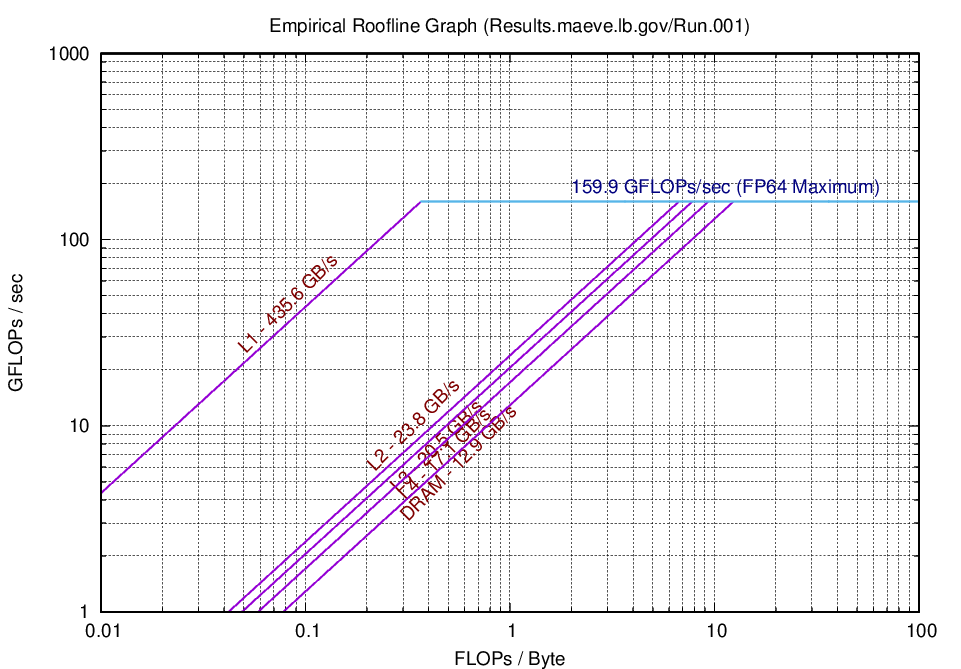
\includegraphics[width=4in]{./imagenes/RTK_ALVARO.png}


\end{frame}

\begin{frame}
    \frametitle{Características del Hardware y del Software}
    Compilador: gcc (Ubuntu 9.3.0-17ubuntu1~20.04) 9.3.0 \\
    OS: Ubuntu 20.04.2 LTS (Focal Fossa) \\
    Arquitectura: x86\_64
\end{frame}


\begin{frame}
    \frametitle{Optimizaciones}

    Primero elegimos un conjunto de flags óptimas \pause
    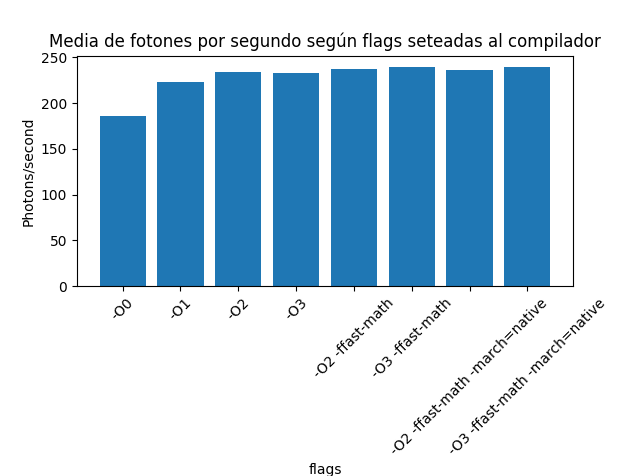
\includegraphics[width=3in]{./imagenes/comparacion_flags_sin_optimizar.png}

\end{frame}

\begin{frame}
    \frametitle{Optimizaciones}

    Fragmento de código a optimizar \\
    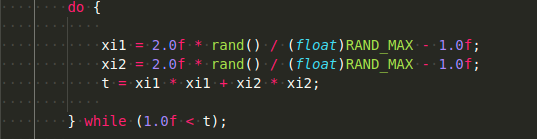
\includegraphics[width=4in]{./imagenes/dowhile_optimizar.png}

\end{frame}

\begin{frame}
    \frametitle{Optimizaciones}
    ¿Qué es lo que hace este código? \\ \pause
    \begin{center}
        $xi1, xi2  \in [-1, 1] $ \\ \pause
        $t = (xi1)^2 + (xi2)^2$ \\ \pause
        i.e $ t \in [0,1]$
    
    \end{center}

\end{frame}


\begin{frame}
    \frametitle{Optimizaciones}
    \begin{center}
        $ t <= 1 $ \\\pause
        $(xi1)^2 + (xi2)^2 <= 1$ \\\pause
        $(xi2)^2 <= 1 - (xi1)^2$ \\\pause
        $xi2 <= \sqrt{1 - (xi1)^2}$\\\pause
        i.e $xi1 \in [0, 1]$\\
        $xi2 \in [0, \sqrt{1 - (xi1)^2}]$    

    \end{center}

\end{frame}

\begin{frame}
    \frametitle{Optimizaciones}

    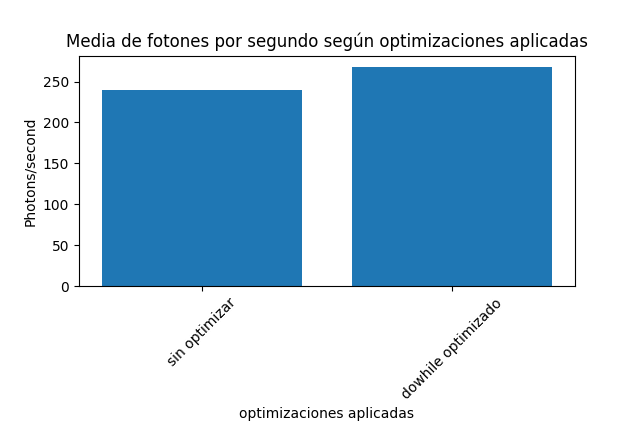
\includegraphics[width=4in]{imagenes/optimizaciones_1.png}
\end{frame}

\begin{frame}
    \frametitle{Optimizaciones}
        Reemplazamos rand() por una implementación de Mersenne Twister en puro C\\\pause
        https://github.com/ESultanik/mtwister
\end{frame}

\begin{frame}
    \frametitle{Optimizaciones}
    
\end{frame}

\begin{frame}
    \frametitle{Optimizaciones}

\end{frame}

\begin{frame}
    \frametitle{Optimizaciones}

\end{frame}


\end{document}